\documentclass[12pt]{article}

\usepackage[utf8]{inputenc}
\usepackage{geometry}
\geometry{a4paper,scale=0.75}
\linespread{1.5}
\usepackage{graphicx} 
\usepackage{float} 
\usepackage{subfig} 
\usepackage{enumerate}
\usepackage{enumitem}
\usepackage{amsmath}
\usepackage{array}
\usepackage{booktabs}
\usepackage{multirow}
\usepackage{amsfonts}
\usepackage[english]{babel}
\usepackage{amsthm}
\usepackage{dcolumn}
\usepackage{multicol}
\usepackage{stfloats}
\usepackage{lscape}
\usepackage[figuresright]{rotating}
\RequirePackage{pdflscape}
\usepackage[toc,page]{appendix}
\usepackage{geometry}
\usepackage{longtable}
\usepackage{comment}
\usepackage{xcolor}

\usepackage{tikz}
\usepackage{pgfplots}
\pgfplotsset{compat=1.18}

% -------- enumerated sub-labels (a), (b), … --
\usepackage{enumitem}
\setlist[enumerate,1]{label=(\alph*),ref=\alph*}
% ---------------------------------------------

\usepackage{hyperref}
\hypersetup{hidelinks,
	colorlinks=true,
	allcolors=black,
	pdfstartview=Fit,
	breaklinks=true}
\usepackage{csquotes}
\usepackage{natbib}
\bibliographystyle{apalike}
\newtheorem{definition}{Definition}
\newtheorem{theorem}{Theorem}
\newtheorem{proposition}[theorem]{Proposition}
\newtheorem{lemma}[theorem]{Lemma}
\newtheorem{corollary}[theorem]{Corollary}
\newtheorem*{remark}{Remark}
\newtheorem{example}{Example}
\newtheorem{exercise}{Exercise}
\newtheorem{assumption}{Assumption}[section] % number within sections


\begin{document}

\thispagestyle{empty}

\begin{center}
    THE HONG KONG UNIVERSITY OF SCIENCE AND TECHNOLOGY\\
    {\large \textbf{ECON 3123 Final Exam}}\\
    Date: Dec 10, 2025\\
    Time allowed: 120 minutes
\end{center}

\vspace{12pt}
\paragraph{Not to be taken away.}
\paragraph{Instructions:}
\begin{itemize}
    \item Answer ALL the questions. Write your answers on the answer book. Anything written on the question book will NOT be graded.
    \item  Use one separate page for each question, and separate subquestions within one question by 1 to 2 blank lines. 
    \item Make sure that all your handweritngs are legible. Anything that cannot be understood by the grader will not be graded. 
    \item Make sure that your answer is clear and concise. Please only write within the area provided for the question. No answer outside the area will be graded.
    \item Please submit BOTH the question book and the answer book after the exam.
\end{itemize}

\vspace{24pt}
\begin{center}
    \Large
    \textbf{DO NOT OPEN UNTIL INSTRUCTED!}
\end{center}

\vspace{24pt}
\subsection*{Name:}
\subsection*{Student ID: }

\clearpage
\setcounter{page}{1}

\noindent\textbf{Question 1: Yield curve and bond pricing (10 points)}

Here is the yield curve of a zero-coupon bond with face value 100.
    \begin{figure}[h!]
        \centering
        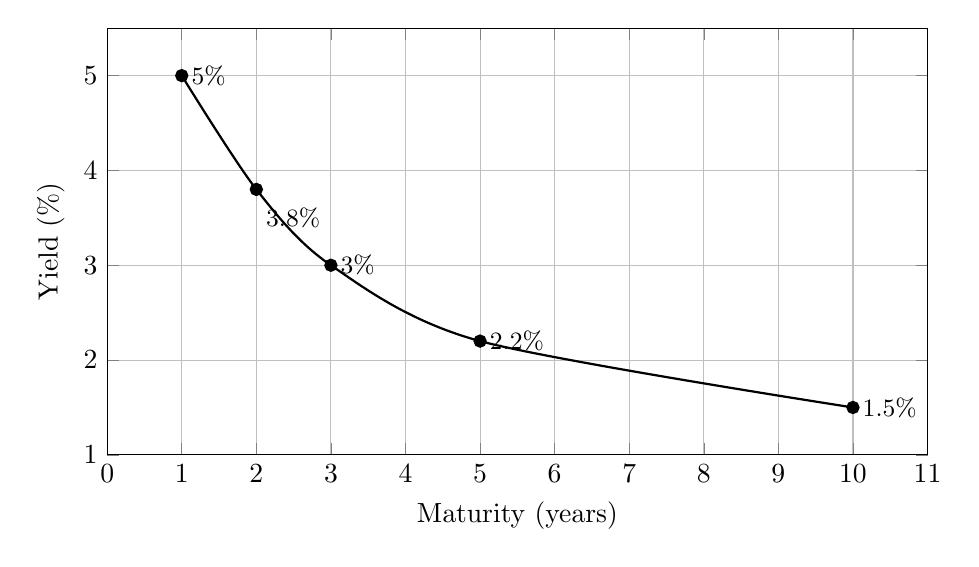
\begin{tikzpicture}
        \begin{axis}[
            width=12cm,
            height=7cm,
            xmin=0, xmax=11,
            ymin=1, ymax=5.5,
            xlabel={Maturity (years)},
            ylabel={Yield (\%)},
            grid=both,
            tick label style={/pgf/number format/fixed},
        ]
        
        % Smooth yield curve with labels
        \addplot[
            smooth,
            thick,
            mark=*,
        ]
        coordinates {
            (1, 5.0)
            (2, 3.8)
            (3, 3.0)
            (5, 2.2)
            (10, 1.5)
        };
        
        % Labels for the points
        \addplot[
            only marks,
            mark=none,
            point meta=explicit symbolic,
            nodes near coords,
            nodes near coords style={font=\small, anchor=west},
        ]
        coordinates {
            (1, 5.0) [5\%]
            (2, 3.5) [3.8\%]
            (3, 3.0) [3\%]
            (5, 2.2) [2.2\%]
            (10, 1.5) [1.5\%]
        };
        
        \end{axis}
        \end{tikzpicture}
    \end{figure}

    Consider the 3-year zero-coupon bond.
\begin{enumerate}[label=(\arabic*)]
    \item (6 points) Assume that the risk premium is constant at 2\%. If the 1-year bond rate does not change, what should it be?
    \item (4 points) According to the graph, do you predict that 
\end{enumerate}

\newpage
\noindent\textbf{Question 2: Productivity shock in the medium run (29 points)}

Suppose that the production function is 
\[Y = \mathcal{A} \sqrt{N},\]
where $Y$ is output, $\mathcal{A}$ is productivity, and $N$ is labour input.

\begin{enumerate}[label=(\arabic*)]
    \item (4 points) Derive the price setting equation. (Hint: The derivative of $\sqrt{x}$ will be $\frac{1}{2\sqrt{x}}$.)
\end{enumerate}

Normalize the total labour force to be $L=1$. Suppose that the wage setting equation is
\[\frac{W}{P^e} = \mathcal{A}(1-\alpha u + z),\]
where $W$ is the nominal wage, $P^e$ is the expected price level, $\alpha\in(0,1)$ is a constant, $u$ is the unemployment rate, and $z$ is the variable capturing all other factors.

\begin{enumerate}[label=(\arabic*),resume]
    \item (6 points) Suppose there is a positive productivity shock, that is, $\mathcal{A}$ increases. Use a \textbf{labour market diagram} (the unemployment-real wage diagram) to illstrate how the equilibrium real wage changes. 
    \item (4 points) Derive the Phillips curve.
    \item (3 points) Derive the PC relation.
    \item (6 points) Assume that after the positive productivity shock, the new short run equilibrium output is higher than the new medium run equilibrium. Use an $IS-LM-PC$ diagram to illustrate the short-run effect on inflation $\pi$, investment $I$, and real interest rate $r$.
    \item (6 points) To stabilize the output, what should the central bank do? Use the same diagram in the previous question to compare the resulting inflation $\pi$, investment $I$, and real interest rate $r$ of your monetary policy with the initial equilibrium (before the shock.)
\end{enumerate}


\newpage
\noindent\textbf{Question 3: Fixed exchange rate regime (24 points)}

Suppose that the economy is summarized by the following equations:
\begin{itemize}
    \item $IS$ curve:
    \[Y = 20-2i.\]
    \item Real interest rate:
    \[\epsilon = E \frac{P}{P^*}.\]
    \item Uncovered interest parity:
    \[1 + i_t = (1 + i^*_t)\frac{E}{\bar{E}^e}.\]
\end{itemize}
Assume that in the short run prices are given so that $\epsilon = E$. The economy is operating under a fixed exchange rate regime at $E = 0.5$. The initial domestic interest rate is 1\%.
\begin{enumerate}[label=(\arabic*)]
    \item (5 points) Use an $IS-LM-UIP$ diagram to represent the economy. Denote the initial equilibrium point by $A$, and label all the curves with subscript $A$.
\end{enumerate}
Suppose that the foreign economy has a negative shock so that its central bank decreases its nominal interest rate to $i^*_B = 0.5\%$ to keep the output $Y^*$ unchanged.
\begin{enumerate}[label=(\arabic*),resume]
    \item (7 points) In the same diagram drawn in (a), show how the domestic central bank should respond in order to keep the exchange rate fixed. Denote the new equilibrium by point $B$. If you shift any curve, label the new curve with subscript $B$.
\end{enumerate}

Due to the decrease in $i^*$, the international investors expect the domestic economy is going to revalue its currency. On average, the investors have an expectation of $\bar{E}^e = 0.8$.

\begin{enumerate}[label=(\arabic*),resume]
    \item (8 points) In the same diagram drawn in (a), show that the central bank cannot maintain a fixed exchange rate regime.If you shift any curve, label the new curve with subscript $C$. You need some tiny math to solve this part.
    \item (4 points) Suppose now the domestic central bank gives up the absolute fixed exchange rate regime but an interval of exchange rates. Find the largest lower bound for this interval.
\end{enumerate}


\newpage
\noindent\textbf{Question 4: Neoclassical Harrod-Domar Model (25 points)}

Suppose that there are $J$ firms, each indexed with $j = 1, 2, \cdots, J$. Each firm $j$ produces output $y_j$ according to the following production function
\[y_j = \bar{A}k_j^{\alpha}N_j^{1-\alpha},\]
where $\bar{A}$ is the constant productivity, $k_j$ is the capital input and $N_j$ is the labour input used by firm $j$, and $\alpha\in(0,1)$. 

The aggregate productivity depends upon the total amount of capital that has been accumulated by all firms:
\[\bar{A} = A_0\left(\sum^{J}_{j=1} k_j\right)^{\eta},\]
where $\eta\in(0,1)$.

Normalize $N_j = 1$ for all $j$. Let $K$ be the aggregate capital such that $K = \sum^{J}_{j=1} k_j$ and $Y$ be the aggregate output such that $Y = \sum^{J}_{j=1} y_j$. Assume that $k_j = \frac{K}{J}$.

Let $s$ denote the saving rate and $\delta$ denote the depreciation rate. The law of motion of capital is
\[K_{t+1} = s Y_t + (1 - \delta) K_t.\]

\begin{enumerate}[label=(\arabic*)]
    \item (6 points) Write aggregate output $Y$ as a function of $K$. You should be able to obtain a form of $Y = A K^{\beta}$ for some $A>0$ and $\beta>0$.
    \item (6 points) Derive the closed-form solution for the steady-state aggregate capital $K_{ss}$.
    \item (5 points) Find the golden-rule level of saving rate $s_G$ when $\beta=0.5$.
    \item (4 points) Write the steady-state growth rate of the economy $g_{ss}$ as a function of $K$. 
    \item (4 points) Derive the condition under which there will be positive growth when $K > K_{ss}$.
\end{enumerate}

\newpage
\noindent\textbf{Question 5: Speculation in foreign exchange market (12 points)}

In class, we learnt the uncovered interest parity. However, it may not hold in reality because there are always fluctuations in the foreign exchagne rate that you cannot predict. 

In order to hedge the risks, the market invented a contract called \textbf{forward}. The idea of the forward contract is as follows. Suppose you hold US dollar (USD) and would like to buy some British pound (GBP) in 1 year. By signing a forward contract today, you will be able to buy the GBP at a specified exchange rate at the maturity date, in this case, 1 year later. Suppose that the forward contract specifies an exchange rate of 1.5 USD/GBP. Then, 1 year later, even the actual exchange rate is ridiculously high at 15 USD/GBP, you can still make the exchange at 1.5 USD/GBP.

From the example, you may already realize that if the forward rate is not deliberately set, there will be opportunities for arbitrage. This question asks you to implement the no-arbitrage condition to calculate the forward rate, and to investigate the opportunities for speculation.

Suppose that the 1-year zero-coupon risk-free US bond has 2\% return, and the  1-year zero-coupon risk-free British bond has 1\% return. The current exchange rate is 1.3 USD/GBP.

\begin{enumerate}[label=(\arabic*)]
    \item (4 points) Using the no-arbitrage condition, derive the forward exchange rate.
    \item (8 points) Suppose that the forward exchange rate is what you have calculated in part (1), but you are really confident that the exchange rate will turn out to be 1.25 USD/GBP. If you are allowed to borrow 1,300,000 USD or, equivalently 1,000,000 GBP now, which one would you choose to make a profit via speculation? What is your strategy? How much will be your profit in terms of the currency you initially borrowed?
\end{enumerate}
\vspace{36pt}
\begin{center}
    \textbf{\Large ******** END OF THE EXAM ********}
\end{center}

\end{document}